\documentclass[twoside]{article}
\usepackage{amsmath}
\usepackage{amssymb}
\usepackage{amsthm}
\usepackage{calc}
\usepackage{capt-of}
\usepackage{caption}
\usepackage[strict]{changepage}
\usepackage{chngcntr}
\usepackage[americanvoltage,siunitx]{circuitikz}
\usepackage{color,colortbl}
\usepackage{etoolbox}
\usepackage{fancyhdr}
\usepackage[T1]{fontenc}
\usepackage{gensymb}
\usepackage[margin=1in]{geometry}
\usepackage{graphicx}
\usepackage{hyperref}
\usepackage{import}
\usepackage{indentfirst}
\usepackage{mathptmx}
\usepackage{mathrsfs}
\usepackage{multicol}
\usepackage{multirow}
\usepackage{needspace}
\usepackage{pgfplots}
\usepackage{pgfplotstable}
\usepackage{setspace}
\usepackage{siunitx}
\usepackage{tabu}
\usepackage{tabularx}
\usepackage{tikz}
\usepackage{xspace}

\patchcmd{\thebibliography}{\section*{\refname}}{\vspace{-1em}}{}{}

\captionsetup{labelformat=empty,labelsep=none}
\usepgfplotslibrary{external}
\usetikzlibrary{positioning,matrix,shapes,chains,arrows}
\tikzexternalize[prefix=precompiled_figures/]

\newcommand\svgsize[2]{\def\svgwidth{#2}
{\centering\input{#1.pdf_tex}}}
\newcommand\svgc[1]{\svgsize{#1}{\columnwidth}}
\newcommand\svgl[1]{\svgsize{#1}{1em}}
\newcommand\diagrams[0]{\renewcommand\svgsize[2]{\def\svgwidth{##2}
{\centering\input{diagrams/##1.pdf_tex}}}}

\newcommand\pdf[1]{\noindent\includegraphics[width=\columnwidth]{#1.pdf}}
\newcommand\pdfex[1]{\pdf{#1}

\pdf{#1ex}}
\newcommand\pdfmsg[1]{\noindent\begin{minipage}{\columnwidth}\pdf{#1msg}

\pdf{#1}\end{minipage}}
\newcommand\pdfmsgex[1]{\pdfmsg{#1}

\pdf{#1ex}}
\newcommand\code[0]{\renewcommand\pdf[1]{\noindent
\includegraphics[width=\columnwidth]{code/##1.pdf}}}

% Indent
\setlength{\parindent}{0.3in}

\newcounter{paperthmamount}
\newcommand\theorems[0]{
\theoremstyle{remark}
\newtheorem{claim}[subsection]{Claim}
\theoremstyle{plain}
\newtheorem{conjecture}[subsection]{Conjecture}
\theoremstyle{plain}
\newtheorem{corollary}[subsection]{Corollary}
\theoremstyle{definition}
\newtheorem{definition}[subsection]{Definition}
\theoremstyle{plain}
\newtheorem{lemma}[subsection]{Lemma}
\theoremstyle{remark}
\newtheorem{proposition}[subsection]{Proposition}
\theoremstyle{remark}
\newtheorem{remark}[subsection]{Remark}
\theoremstyle{plain}
\newtheorem{theorem}[subsection]{Theorem}
\theoremstyle{definition}
\newtheorem{question}[subsection]{Question}
\newcommand\paperclm[2]
{\begin{claim}\global\expandafter\edef
\csname clm##1\endcsname{Claim \thesubsection\noexpand\xspace}
##2\end{claim}}
\newcommand\papercnj[2]
{\begin{conjecture}\global\expandafter\edef
\csname cnj##1\endcsname{Conjecture \thesubsection\noexpand\xspace}
##2\end{conjecture}}
\newcommand\papercor[2]
{\begin{corollary}\global\expandafter\edef
\csname cor##1\endcsname{Corollary \thesubsection\noexpand\xspace}
##2\end{corollary}}
\newcommand\paperdef[2]
{\begin{definition}\global\expandafter\edef
\csname def##1\endcsname{Definition \thesubsection\noexpand\xspace}
##2\end{definition}}
\newcommand\paperlem[2]
{\begin{lemma}\global\expandafter\edef
\csname lem##1\endcsname{Lemma \thesubsection\noexpand\xspace}
##2\end{lemma}}
\newcommand\paperprp[2]
{\begin{proposition}\global\expandafter\edef
\csname prp##1\endcsname{Proposition \thesubsection\noexpand\xspace}
##2\end{proposition}}
\newcommand\paperqtn[2]
{\begin{question}\global\expandafter\edef
\csname qtn##1\endcsname{Question \thesubsection\noexpand\xspace}
##2\end{question}}
\newcommand\paperrem[2]
{\begin{remark}\global\expandafter\edef
\csname rem##1\endcsname{Remark \thesubsection\noexpand\xspace}
##2\end{remark}}
\newcommand\paperthm[2]
{\begin{theorem}\global\expandafter\edef
\csname thm##1\endcsname{Theorem \thesubsection\noexpand\xspace}
##2\end{theorem}}}
\newcommand\subtheorems[0]{\stepcounter{paperthmamount}
\theoremstyle{remark}
\newtheorem{claim}[subsubsection]{Claim}
\theoremstyle{plain}
\newtheorem{conjecture}[subsubsection]{Conjecture}
\theoremstyle{plain}
\newtheorem{corollary}[subsubsection]{Corollary}
\theoremstyle{definition}
\newtheorem{definition}[subsubsection]{Definition}
\theoremstyle{plain}
\newtheorem{lemma}[subsubsection]{Lemma}
\theoremstyle{remark}
\newtheorem{proposition}[subsubsection]{Proposition}
\theoremstyle{remark}
\newtheorem{remark}[subsubsection]{Remark}
\theoremstyle{plain}
\newtheorem{theorem}[subsubsection]{Theorem}
\theoremstyle{definition}
\newtheorem{question}[subsubsection]{Question}
\newcommand\paperclm[2]
{\begin{claim}\global\expandafter\edef
\csname clm##1\endcsname{Claim \thesubsubsection\noexpand\xspace}
##2\end{claim}}
\newcommand\papercnj[2]
{\begin{conjecture}\global\expandafter\edef
\csname cnj##1\endcsname{Conjecture \thesubsubsection\noexpand\xspace}
##2\end{conjecture}}
\newcommand\papercor[2]
{\begin{corollary}\global\expandafter\edef
\csname cor##1\endcsname{Corollary \thesubsubsection\noexpand\xspace}
##2\end{corollary}}
\newcommand\paperdef[2]
{\begin{definition}\global\expandafter\edef
\csname def##1\endcsname{Definition \thesubsubsection\noexpand\xspace}
##2\end{definition}}
\newcommand\paperlem[2]
{\begin{lemma}\global\expandafter\edef
\csname lem##1\endcsname{Lemma \thesubsubsection\noexpand\xspace}
##2\end{lemma}}
\newcommand\paperprp[2]
{\begin{proposition}\global\expandafter\edef
\csname prp##1\endcsname{Proposition \thesubsubsection\noexpand\xspace}
##2\end{proposition}}
\newcommand\paperqtn[2]
{\begin{question}\global\expandafter\edef
\csname qtn##1\endcsname{Question \thesubsubsection\noexpand\xspace}
##2\end{question}}
\newcommand\paperrem[2]
{\begin{remark}\global\expandafter\edef
\csname rem##1\endcsname{Remark \thesubsubsection\noexpand\xspace}
##2\end{remark}}
\newcommand\paperthm[2]
{\begin{theorem}\global\expandafter\edef
\csname thm##1\endcsname{Theorem \thesubsubsection\noexpand\xspace}
##2\end{theorem}}}

% Title section
\pagestyle{fancy}
\thispagestyle{empty}
\renewcommand{\headrulewidth}{0pt}
\newcommand\papertitle[1]
{{\centering\fontsize{20pt}{20pt}\textsc{#1}\\\mbox{}\\}
\fancyhead[OC]{\fontsize{12pt}{12pt}\selectfont\textit{#1}}}
\newcounter{people}
\newcommand\paperauthtext[3]{{\centering\fontsize{12pt}{12pt}\selectfont
\textsc{#1}\\[-0.1em]{\fontsize{9pt}{9pt}\selectfont\textit{\ifx&#2&
\vspace{-1em}\else#2\fi}}\\\mbox{}\\
\fancyhead[EC]{\fontsize{12pt}{12pt}\selectfont\textit{#3}}}}
\newcommand\paperauth[2]{{\stepcounter{people}
\ifnum\value{people}=1
{\paperauthtext{#1}{#2}{#1}
\global\def\auth{#1\xspace}}
\else\ifnum\value{people}=2
{\paperauthtext{#1}{#2}{\auth and #1}}
\else{\paperauthtext{#1}{#2}{\auth et al}}\fi\fi}}
\newcommand\physics[0]{
\renewcommand\paperauthtext[4]{{\centering\fontsize{12pt}{12pt}\selectfont
\textsc{##1. ##2}\\[-0.1em]{\fontsize{9pt}{9pt}\selectfont\textit{\ifx&##3&
\vspace{-1em}\else##3\fi}}\\\mbox{}\\
\fancyhead[EC]{\fontsize{12pt}{12pt}\selectfont\textit{##4}}}}
\renewcommand\paperauth[3]{{\stepcounter{people}
\ifnum\value{people}=1
{\paperauthtext{##1}{##2}{##3}{##1. ##2}
\global\def\auth{##2\xspace}}
\else\ifnum\value{people}=2
{\paperauthtext{##1}{##2}{##3}{\auth and ##2}}
\else{\paperauthtext{##1}{##2}{##3}{\auth et al}}\fi\fi}}}
\newcommand\paperdate[1]{{\centering\fontsize{9pt}{9pt}\selectfont\text{
(Received #1)}\\[2em]}}

% Page header
\newcommand{\paperhead}[1]{\fancyhead[EC]{\fontsize{12pt}{12pt}\selectfont
\textit{#1}}}
\fancyhead[RO, EL]{\fontsize{12pt}{12pt}\selectfont\thepage}
\fancyhead[RE, OL]{}
\cfoot{}

\makeatletter
\newenvironment{paperadjustwidth}[2]{
  \begin{list}{}{
    \setlength\partopsep\z@
    \setlength\topsep\z@
    \setlength\listparindent\parindent
    \setlength\parsep\parskip
    \@ifmtarg{#1}{\setlength{\leftmargin}{\z@}}
                 {\setlength{\leftmargin}{#1}}
    \@ifmtarg{#2}{\setlength{\rightmargin}{\z@}}
                 {\setlength{\rightmargin}{#2}}
    }
    \item[]}{\end{list}}
\makeatother

%Figure counter
\newcounter{paperfigurecounter}
\newcommand{\papercap}[2]{\bgroup\stepcounter{paperfigurecounter}
\captionof{figure}{\fontsize{9pt}{9pt}\selectfont
\hspace{0.3in}Fig.~\arabic{paperfigurecounter}.\quad#2}
\egroup\expandafter\edef
\csname fig#1\endcsname{Fig.~\arabic{paperfigurecounter}\noexpand\xspace}}

\newcommand\paperfig[3]{\noindent\begin{minipage}{\columnwidth}
#2\papercap{#1}{#3}\end{minipage}\expandafter\edef
\csname fig#1\endcsname{Fig.~\arabic{paperfigurecounter}\noexpand\xspace}}
\newcommand\papersvg[3]{\paperfig{#1}{\svgc{#2}}{#3}}

% Abstract environment
\newenvironment{paperabs}
{\begin{paperadjustwidth}{0.5in}{0.5in}\bgroup\fontsize{9pt}{9pt}\selectfont
\hspace{0.5in}}
{\egroup\end{paperadjustwidth}}

% Paper environment
\setlength\columnsep{0.5in}
\newenvironment{paper}
{\begin{multicols*}{2}\bgroup\fontsize{12pt}{12pt}\selectfont}
{\egroup\end{multicols*}}
\newcommand{\singlecolumn}[0]{
\renewcommand\paperfig[3]{\noindent
\makebox[\textwidth][c]{\begin{minipage}{5.5in}
\noindent\makebox[\textwidth][c]{\begin{minipage}{3in}##2\end{minipage}}
\papercap{##1}{##3}\end{minipage}}\expandafter\edef
\csname fig##1\endcsname{Fig.~\arabic{paperfigurecounter}\noexpand\xspace}}
\renewenvironment{paper}{\bgroup\fontsize{12pt}{12pt}\selectfont}
{\egroup}}

%Sources
\newsavebox{\sourcebox}
\newcommand{\papersource}[1]{
\vspace{-2em}
\text{}\\*
\fontsize{9pt}{9pt}\selectfont
\noindent\renewcommand{\labelenumi}{}
\savebox{\sourcebox}{\parbox{3in}{\begin{enumerate}
\setlength{\leftmargini}{-1ex}
\setlength{\leftmargin}{-1ex}
\setlength{\labelwidth}{0pt}
\setlength{\labelsep}{0pt}
\setlength{\listparindent}{0pt}
\item\textit{\hspace{-0.35in}#1}
\end{enumerate}}}
\usebox{\sourcebox}
}

%Section headers
\newcounter{paperseccounter}
\newcounter{papersubseccounter}[paperseccounter]
\newcommand\papersec[1]{\needspace{1in}
\stepcounter{paperseccounter}
\stepcounter{section}
\begin{center}\Roman{paperseccounter} \textsc{#1}\end{center}}
\newcommand\papersubsec[1]{\needspace{1in}
\stepcounter{papersubseccounter}
\addtocounter{subsection}{\thepaperthmamount}
\setcounter{subsubsection}{0}
{\begin{center}
\Roman{section}.\Roman{papersubseccounter}
\textsc{#1}\\[0.5em]\end{center}}}

%equation
\newcounter{papereqcounter}
\newcommand\papereq[3]{{
\stepcounter{papereqcounter}
\mbox{}\vspace{-0.75em}
\begin{equation*}
#2
\tag*{\fontsize{12pt}{12pt}\selectfont
$\begin{array}{r}
\cr{\text{(\arabic{papereqcounter})}}
\cr{\fontsize{9pt}{9pt}\selectfont\textit{\ifx\\#3\\~\else(\fi#3\ifx\\#3\\~
\else)\fi}}
\end{array}$}
\end{equation*}

}
\expandafter\edef\csname eq#1\endcsname{(\arabic{papereqcounter})\noexpand
\xspace}}

% Where
\newcommand{\papervar}[3]
{&$#1$ & #2 \ifx\\#3\\~\else($\smash{\text{\si{\fi
#3\ifx\\#3\\~\else}}}$)\fi\\}
\newenvironment{paperwhere}
{\begin{minipage}{\columnwidth}
\bgroup\fontsize{9pt}{9pt}\selectfont Where:\vspace{2pt}\\\begin{tabular}
{rr@{ = }p{\linewidth}}}
{\end{tabular}\egroup\end{minipage}\vspace{5pt}}

% Tables
\definecolor{LineGray}{gray}{0.5}
\newtabulinestyle{outer=2.25pt LineGray}
\newtabulinestyle{inner=0.75pt LineGray}
\tabulinesep=1.5pt

\newcommand{\paperiline}[0]{\tabucline[inner]{-}}
\newcommand{\paperoline}[0]{\tabucline[outer]{-}}

% Index column type
\newcolumntype{I}{X[-5,c]}
% Column type with uncertainty
\newcolumntype{U}{@{}X[-5,r]@{$\pm$}X[-5,l]@{}}
% Column type without uncertainty
\newcolumntype{C}{@{}X[-5,c]@{}}

\newcounter{papertableindexcounter}
\newcommand{\papertableindexheader}[0]{\multirow{2}{*}{\textsc{Index}}}
\newcommand{\papertableindex}[0]{\stepcounter{papertableindexcounter}
\arabic{papertableindexcounter}}
\newcommand{\papertableuheadersymbol}[1]{&\multicolumn{2}{c|[inner]}{$#1$}}
\newcommand{\papertableuheadersymbole}[1]{&\multicolumn{2}{c|[outer]}{$#1$}}
\newcommand{\papertableuheaderunit}[1]{&\multicolumn{2}{c|[inner]}{(#1)}}
\newcommand{\papertableuheaderunite}[1]{&\multicolumn{2}{c|[outer]}{(#1)}}
\newcommand{\papertablecheadersymbol}[1]{&$#1$}
\newcommand{\papertablecheaderunit}[2]{&($\pm$#1 #2)}

% Value in table with uncertainty.
\newcommand{\papertableuval}[2]{& #1 & #2}
% Value in table without uncertainty.
\newcommand{\papertablecval}[1]{& #1}

\newenvironment{papertable}[1]
{\setcounter{papertableindexcounter}{0} 
\begin{tabu} to \linewidth {#1}}
{\end{tabu}\vspace{12pt}}

\newcommand{\paperaxis}[9]
{title=#1,
axis x line = bottom,
xmin=#4,xmax=#6,
axis y line = left,
ymin=#5,ymax=#7,
height = 180pt,
grid=both,
x axis line style=-,
y axis line style=-,
x tick label style={
/pgf/number format/.cd,
fixed,
fixed zerofill,
precision=#8,
/tikz/.cd},
y tick label style={
/pgf/number format/.cd,
fixed,
fixed zerofill,
precision=#9,
/tikz/.cd}}
\newcommand{\paperaxisxlabel}[2]{
xlabel=\fontsize{10pt}{10pt}\selectfont#1$(#2)\rightarrow$}
\newcommand{\paperaxisylabel}[2]{
ylabel=\fontsize{10pt}{10pt}\selectfont#1$(#2)\rightarrow$}
\newcommand{\papergraphoutline}[4]{
\addplot [mark=none,line width=0.75pt] coordinates {
(#1,#2)
(#1,#4)
(#3,#4)
(#3,#2)
(#1,#2)};}

\newenvironment{papergraph}{
\begin{tikzpicture}
\begin{axis}}
{\end{axis}
\end{tikzpicture}}

\newcommand{\comment}[1]{}

\newcommand{\abs}[1]{\left\lvert#1\right\rvert}
\newcommand{\oo}[0]{\infty}
\newcommand{\sigmaSum}[3]{\sum\limits_{#1}^{#2} #3}
\newcommand{\limto}[3]{\lim\limits_{#1\rightarrow#2}#3}
\renewcommand{\d}[0]{\mathrm{d}}
\newcommand{\cross}[0]{\times}
\newcommand{\lp}{\left(}
\newcommand{\rp}{\right)}
\newcommand\pars[1]{\lp#1\rp}
\newcommand\sqbrack[1]{\left[#1\right]}
\newcommand\R{\mathbb{R}}
\newcommand\di{\partial}
\newcommand\x{\times}
\newcommand\del{\nabla}

\physics
\begin{document}
\papertitle{Analysis of Atomic Spectra of Various Gases}
\paperauth{A}{Khesin}{Lab Technician}
\paperauth{P}{Zavyalova}{Data Analyst}
\paperdate{January 15, 2018}
\begin{paperabs}
TODO Abstract
\end{paperabs}

\begin{paper}
\papersec{Introduction}

The purpose of this experiment was to use a prism spectrometer to identify
unknown gases based on their atomic spectra.
Furthermore, the Rydberg constant ($R_H$) was determined by examining the
spectral lines of hydrogen.
The apparatus consisted of a spectrometer, a sodium lamp, a tube of hydrogen
gas, a tube of helium gas, and two tubes of unknown compounds marked ``Unknown
\#7'' and ``Unknown \#9''.

The spectrometer was calibrated by aligning the eyepiece with the lines produced
by the sodium lamp and the Hartmann relation method was used to determine the
relation between the observed wavelength and the scale reading on the
spectrometer.

By examining the spectral lines of hydrogen, the Rydberg constant was
determined with the following formula.

\papereq{Rydberg}{\frac1\lambda=R_H\pars{\frac14-\frac1{n^2}}}{Serbanescu}
\begin{paperwhere}
\papervar{\lambda}{observed wavelength}{\meter}
\papervar{R_H}{Rydberg constant}{\per\meter}
\papervar{n}{index of spectral line}{}
\end{paperwhere}

To determine the relation between the scale reading of the spectrometer and the
observed wavelength, the Hartmann relation was used.

\papereq{Hartmann}{y=\frac{m}{\lambda-\lambda_0}+b}{Serbanescu}
\begin{paperwhere}
\papervar{y}{scale reading}{}
\papervar{m}{slope of fit}{\meter}
\papervar{\lambda}{observed wavelength}{\meter}
\papervar{\lambda_0}{fundamental wavelength of spectrometer}{\meter}
\papervar{b}{constant of fit}{}
\end{paperwhere}

For the spectrometer used in the experiment, the value of $\lambda_0$ was
provided as $(285.2\pm.4)\si{\nano\meter}$.

The experiment was setup as shown.
\paperfig{Setup}{\pdf{setup}}{The experimental setup.
The spectrometer (left) is pointing at a tube containing ``Unknown \#7'' (right).}
\papersec{Observations}

The vernier scale on the spectrometer had a reading error of
$\pm.02\si{\nano\meter}$.
The uncertainties in the wavelengths for the spectral lines of helium were
deemed too small to consider.

The vernier scale readings were recorded for helium, hydrogen, ``Unknown \#7'',
and ``Unknown \#9''.
Additionally, the colours of the observed lines and matched wavelengths for the
spectral lines of helium were recorded.

\paperfig{Helium}{\begin{papertable}{|[outer]I|[inner]C|[inner]C|[inner]C|[outer]}
\paperoline\papertableindexheader&\textsc{Scale}&\textsc{Wavelength}&\multirow{2}{*}{\textsc{Colour}}\\
\papertablecheaderunit{.02}{\hspace{-0.5ex}}\papertablecheadersymbol{\lambda~(\si{\nano\meter})}&\\\paperiline
\papertableindex\papertablecval{6.66}\papertablecval{706.5}\papertablecval{Red}\\\paperiline
\papertableindex\papertablecval{7.06}\papertablecval{667.8}\papertablecval{Red}\\\paperiline
\papertableindex\papertablecval{8.31}\papertablecval{587.6}\papertablecval{Yellow}\\\paperiline
\papertableindex\papertablecval{11.09}\papertablecval{501.6}\papertablecval{Green}\\\paperiline
\papertableindex\papertablecval{11.50}\papertablecval{492.2}\papertablecval{Green}\\\paperiline
\papertableindex\papertablecval{12.58}\papertablecval{471.3}\papertablecval{Blue}\\\paperiline
\papertableindex\papertablecval{14.19}\papertablecval{447.1}\papertablecval{Blue}\\\paperoline
\end{papertable}\vspace{-1.5em}}
{The scale readings, matched wavelengths, and colours of the spectral lines of helium.}\vspace{1em}

\paperfig{Hydrogen}{\begin{papertable}{|[outer]I|[inner]C|[inner]C|[inner]C|[outer]}
\paperoline\papertableindexheader&\multirow{2}{*}{\textsc{Line Index}}&\textsc{Scale}&\multirow{2}{*}{\textsc{Colour}}\\
&\papertablecheaderunit{.02}{\hspace{-0.5ex}}&\\\paperiline
\papertableindex\papertablecval{3}\papertablecval{7.26}\papertablecval{Red}\\\paperiline
\papertableindex\papertablecval{4}\papertablecval{11.80}\papertablecval{Blue-Green}\\\paperiline
\papertableindex\papertablecval{5}\papertablecval{15.15}\papertablecval{Violet}\\\paperiline
\papertableindex\papertablecval{6}\papertablecval{17.75}\papertablecval{Violet}\\\paperoline
\end{papertable}\vspace{-1.5em}}
{The scale readings, indices, and colours of the spectral lines of hydrogen.}\vspace{1em}

\paperfig{UnknownSeven}{\begin{papertable}{|[outer]I|[inner]C|[inner]C|[outer]}
\paperoline\papertableindexheader&\textsc{Scale}&\multirow{2}{*}{\textsc{Colour}}\\
\papertablecheaderunit{.02}{\hspace{-0.5ex}}&\\\paperiline
\papertableindex\papertablecval{8.44}\papertablecval{Orange}\\\paperiline
\papertableindex\papertablecval{9.18}\papertablecval{Green}\\\paperiline
\papertableindex\papertablecval{13.89}\papertablecval{Violet}\\\paperiline
\papertableindex\papertablecval{15.38}\papertablecval{Violet}\\\paperoline
\end{papertable}\vspace{-1.5em}}
{The scale readings and colours of the spectral lines of ``Unknown \#7''.}\vspace{1em}

\paperfig{UnknownNine}{\begin{papertable}{|[outer]I|[inner]C|[inner]C|[outer]}
\paperoline\papertableindexheader&\textsc{Scale}&\multirow{2}{*}{\textsc{Colour}}\\
\papertablecheaderunit{.02}{\hspace{-0.5ex}}&\\\paperiline
\papertableindex\papertablecval{TODO}\papertablecval{Red}\\\paperiline
\papertableindex\papertablecval{TODO}\papertablecval{Orange}\\\paperiline
\papertableindex\papertablecval{TODO}\papertablecval{Yellow}\\\paperiline
\papertableindex\papertablecval{TODO}\papertablecval{Green}\\\paperoline
\end{papertable}\vspace{-1.5em}}
{The scale readings and colours of the spectral lines of ``Unknown \#9''.}

\papersec{Analysis}

The relationship between the observed wavelength and the
scale reading on the spectrometer was calculated.
This was done by subtracting $\lambda_0$ from all of the values in the wavelength column of
\figHelium and then taking the reciprocals to get the values of the independent
variables.
All uncertainties were propagated using the method of quadratures.
The scale column formed the values for the dependent variable.
Applying the fit yielded a slope of $(2.00\pm.02)\x\SI{E-6}{\meter}$ and a
y-intercept of $(1.83\pm.09)$.
The $R^2$ value for the fit s 0.999489.
The reduced $ \chi^2 $ obtained is $ 12.5827907379 $ with residuals visualized below.

\paperfig{Residuals}{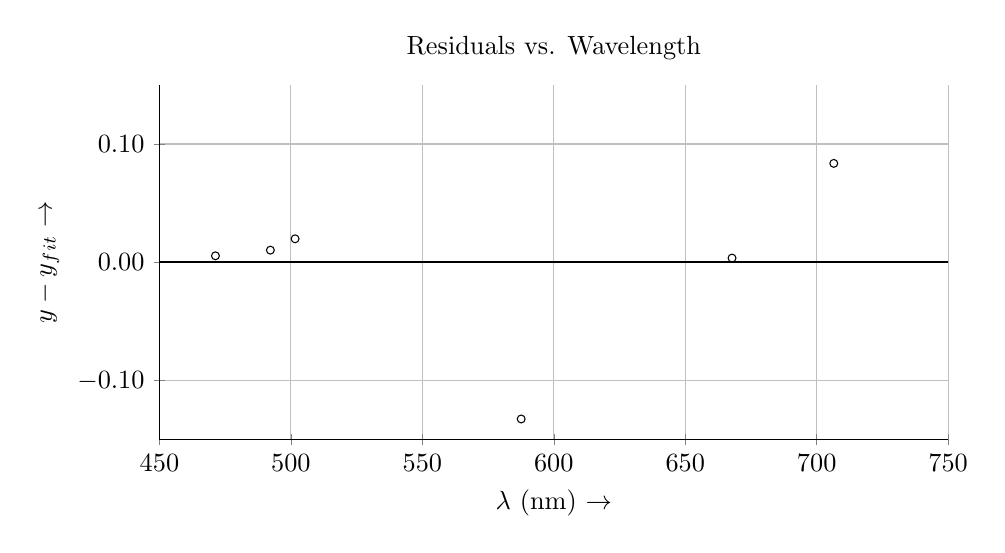
\begin{tikzpicture}[scale = 0.95]
	\begin{axis}
		[width=\linewidth,
		tick label style={font=\fontsize{10pt}{1em}},
		xlabel={\fontsize{10pt}{1em}\selectfont $\lambda$ (\si{\nm}) $\rightarrow$},
		ylabel={\fontsize{10pt}{1em}\selectfont $ y - y_{fit} \rightarrow$},
		\paperaxis{Residuals vs. Wavelength}{y}{x}{450}{-0.15}{750}{0.15}{0}{2}]
		\papergraphoutline{450}{0}{750}{0};
		\addplot[color = black, only marks, mark = o, mark size = 1.5, error bars/.cd,
		y dir = both, y explicit, x dir = both, x explicit] 
		coordinates {
			(706.5, 0.0836354) (667.8, 0.00358039) (587.6, -0.13242233)
			(501.6, 0.01987709) (492.2, 0.01029522) (471.3, 0.00550431)
			(447.1, 0.00952993)
		};
	\end{axis}
\end{tikzpicture}}{WHAT TO ADD HERE?}

\paperfig{ScaleFit}{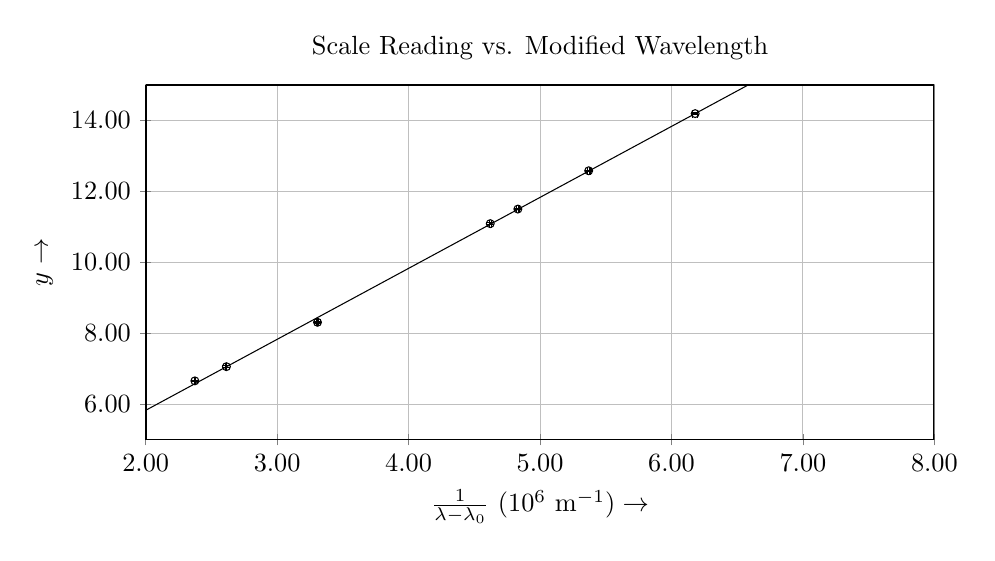
\begin{tikzpicture}[scale=0.95]
\begin{axis}[width=\linewidth,
tick label style={font=\fontsize{10pt}{1em}},
xlabel={\fontsize{10pt}{1em}\selectfont $\frac{1}{\lambda-\lambda_0}$ ($10^6$ $\si{\per\meter})\rightarrow$},
ylabel={\fontsize{10pt}{1em}\selectfont $y\rightarrow$},
\paperaxis{Scale Reading vs. Modified Wavelength}{y}{x}{2}{5}{8}{15}{2}{2}]
\papergraphoutline{2}{5}{8}{15};
\addplot [color=black,only marks,mark=o,mark size=1.5,
error bars/.cd,
y dir=both,y explicit,
x dir=both,x explicit
] coordinates {
(2.374, 6.66) +- (0.002,0.02)
(2.614, 7.06) +- (0.003,0.02)
(3.307, 8.31) +- (0.004,0.02)
(4.621, 11.09) +- (0.009,0.02)
(4.831, 11.50) +- (0.009,0.02)
(5.37, 12.58) +- (0.01,0.02)
(6.18, 14.19) +- (0.02,0.02)
};
\addplot[no marks,
samples=250,
domain=2:8]
{2*x+1.83};
\end{axis}
\end{tikzpicture}}
{The scale readings on the spectrometer plotted against the modified
wavelengths with the line of best fit.
The line has a function of $(2.00\pm.02)\text{E-6}x+(1.83\pm.09)$ and an
\smash{$R^2$} value of 0.999489.
Error bars were included but were too small to be visible.}

Then, \eqHartmann was inverted to convert scale readings into wavelengths.

\papereq{Invert}{\lambda=\frac{m}{y-b}+\lambda_0}{}

By converting all the scale readings from \figHydrogen and plugging the
wavelengths and the line indices into \eqRydberg, four approximations
for the Rydberg constant were obtained.
They were averaged to get the final value for $R_H$, which was
$(1.097\pm.003)\x\SI{E7}{\per\meter}$, which was well within the range of the
experimental error from the accepted $\SI{1.09737316E7}{\per\meter}$.

\papersec{Conclusion}

Conclusion goes here

\papersec{Sources}

\papersource{Serbanescu, R., Measuring atomic spectra, 2014}
\end{paper}
\end{document}